% gr-Paley13.tex -- the Paley graph P(13) : i ~ j when i-j is a square
% modulo 13 (1, 3, 4, 9, 10, 12). Its complement (differences 2, 5, 6)
% is isomorphic to it : the edges of K13 are split into two copies of
% the same graph. Engine : pdfLaTeX or LuaLaTeX
\documentclass[border=3mm, convert=false]{standalone}
\usepackage{tkz-berge}
\begin{document}
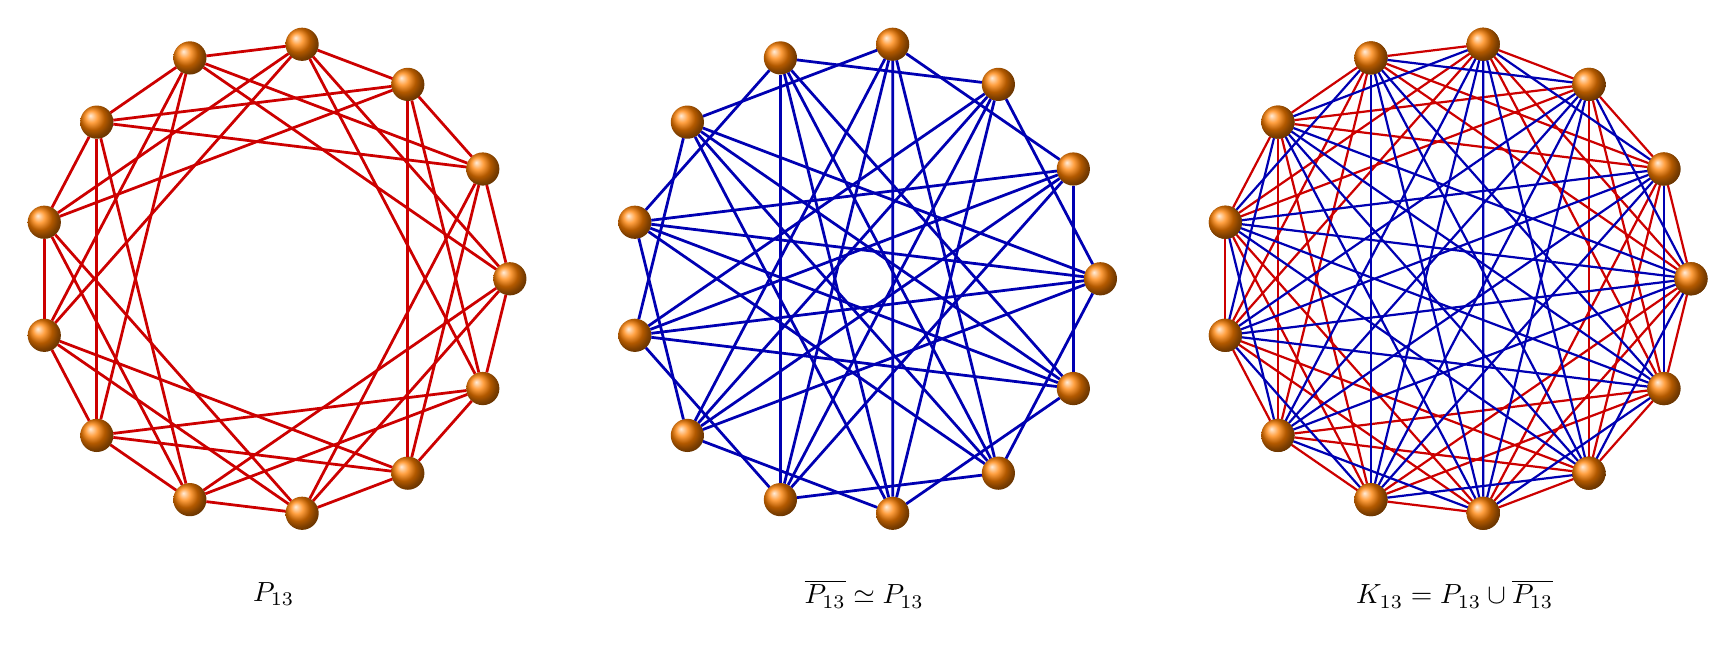
\begin{tikzpicture}
  \GraphInit[vstyle=Art]
  \SetUpEdge[color=red!80!black,lw=1pt]
  \grCirculant[RA=3]{13}{1,3,4}
  \begin{scope}[xshift=7.5cm]
    \SetUpEdge[color=blue!70!black,lw=1pt]
    \grCirculant[RA=3]{13}{2,5,6}
  \end{scope}
  \begin{scope}[xshift=15cm]
    \SetUpEdge[color=red!80!black,lw=.8pt]
    \grCirculant[RA=3]{13}{1,3,4}
    \SetUpEdge[color=blue!70!black,lw=.8pt]
    \grCirculant[RA=3]{13}{2,5,6}
  \end{scope}
  \node at (0,-4)    {\(P_{13}\)};
  \node at (7.5,-4)  {\(\overline{P_{13}}\simeq P_{13}\)};
  \node at (15,-4)   {\(K_{13}=P_{13}\cup\overline{P_{13}}\)};
\end{tikzpicture}
\end{document}
